\section{Induktionsgesetz für Leiterschleifen}

\begin{wrapfigure}[]{l}[0cm]{0cm}
	\raisebox{0pt}[\dimexpr\height-1\baselineskip\relax]{
		\colorbox{hgrey}{
			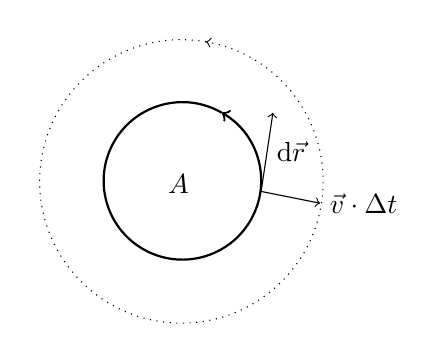
\begin{tikzpicture}
			
			\draw[thick,->] (3.2,0) arc (60:420:1);
			\draw[dotted,->] (3,0.9) arc (80:440:1.8);
			\draw[->] (3.7,-1)--node[right]{$\mathrm{d}\vec{r}$}(3.85,0) ;
			\draw[->] (3.7,-1)--(4.45,-1.15)node[right]{$\vec{v}\cdot\Delta t$} ;
			\draw (2.65,-.9) node{$A$};
			
			
			\end{tikzpicture}
		}
	}
	\caption{Flächenänderung}
\end{wrapfigure}
Zunächst definieren wir den magnetischen Fluss $\Phi$ durch eine Fläche $\vec{A}$ im Raum:

\begin{equation*}
\Phi := \iint\limits_A\mathrm{d}\vec{A}\cdot\vec{B}
\end{equation*}

Man sieht leicht, dass sich der Fluss $\Phi$ bei Flächenänderung und Änderung der magnetischen Flussdichte $\vec{B}$ ändert:\\


\begin{align*}
\Delta\Phi &=  \Delta\left(\iint\mathrm{d}\vec{A}\cdot\vec{B}\right) = \iint\limits_A\mathrm{d}\vec{A}\cdot\Delta\vec{B} \; + \; \iint\limits_{\Delta A}\mathrm{d}\vec{A}\cdot\vec{B}\\
&= \Delta t \iint\limits_A\mathrm{d}\vec{A}\cdot\pdiff{\vec{B}}{t} \; + \; \oint\limits_{\partial A}\left(\vec{v}\Delta t\times\mathrm{d}\vec{r}\right)\cdot\vec{B}\\
&= \Delta t\left(\iint\limits_A\mathrm{d}\vec{V}\cdot\dot{\vec{B}} \; - \; \oint\limits_{\partial A}\mathrm{d}\vec{r}\cdot\left(\vec{v}\times\vec{B}\right)\right)\\
\Rightarrow \dot{\Phi} &= \iint\limits_A\mathrm{d}\vec{A}\cdot\dot{\vec{B}} \; - \; \oint\limits_{\partial A}\mathrm{d}\vec{r} \ \left(\vec{v}\times\vec{B}\right)
\end{align*}

Nach Anwenden der dritten \textsc{Maxwell}-Gleichung erhält man das \textbf{Induktionsgesetz}:
\begin{equation*}
\dot{\Phi} = - \oint\limits_{\partial A}\mathrm{d}\vec{r} \ \left(\vec{E} + \vec{v}\times\vec{B}\right) = - U_{\mathrm{induziert}}
\end{equation*}

Das letzte Minuszeichen nennt man auch die \textbf{\textsc{Lenz}`sche Regel}, welche besagt, dass ein induzierter Strom immer ein Magnetfeld erzeugt, welches seiner eigenen Ursache ($U_{\mathrm{induziert}}$) entgegengerichtet ist.
\ \\
Auffällig bei dem Induktionsgesetz ist seine Ähnlichkeit mit der auf eine freie Ladung wirkende Kraft $\vec{F} = Q(\vec{E} + \vec{v}\times\vec{B})$. Darin liegt auch die Begründung für ebenjenes Gesetz:\

Wir stellen uns eine Leiterschleife vor, welche an einer Stelle durchbrochen ist, damit kein Strom durch die Schleife fließen könnte. Auf einen sich in dieser Schleife bewegenden Ladungsträger wirkt die Kraft:

\begin{equation*}
\vec{F} = Q(\vec{E} + \vec{v}\times\vec{B}) =: Q\vec{E'}
\end{equation*} 

Man sieht, dass das $\vec{E}$-Feld abhängig vom Bezugsystem ist, daher haben wir für $\vec{E'}$ ein Bezugssystem konstruiert, welches sich mit der Geschwindigkeit $\vec{v}$ gegenüber dem Laborsystem bewegt. Damit haben wir im mitbewegeten Bezugssystem erreicht, dass $\vec{v'} = 0$ ist. Bilden wir nun das Weginteral für ein Teilchen entlang der Leiterschleife im $\vec{E}$-Feld erhalten wir:

\begin{equation*}
\oint\limits_{\mathrm{Schleife}}\mathrm{d}\vec{r}\cdot\left(\vec{E} + \vec{v}\times\vec{B}\right) = \oint\limits_{\mathrm{Schleife}}\mathrm{d}\vec{r}\cdot\vec{E'} = \int\limits_{\mathrm{Beginn}}^{\mathrm{Ende}}\mathrm{d}\vec{r}\cdot\vec{E'} = U_{\mathrm{induziert}}
\end{equation*}

\chapter{Elektrostatik}

\section{Grundgleichungen und elektrostatisches Potential}

In der Elektrostatik betrachten wir, wie der Name schon andeutet, zeitunabhängige Felder. Dementsprechend kann man als erste Konsequenz daraus folgern, dass $\dot{\vec{E}} = 0$ und $\dot{\vec{B}} = 0$ ist. Fallen nun in den \textsc{Maxwell}-Gleichungen alle Beiträge mit $\dot{\vec{E}}$ und $\dot{\vec{B}}$ weg, kann man die Felder $\vec{E}$ und $\vec{B}$ getrennt voneinander betrachten. Laienhaft gesprochen entkoppeln wir die Phänomene \grqq Elektrizität\grqq und "Magnetismus". Des Weiteren betrachten wir in der Elektrostatik nur ruhende Ladungen, woraus folgt, dass außerdem $\vec{j}=0 \Rightarrow \vec{B}=0$ ist.\

Damit erhalten wir aus der dritten \textsc{Maxwell}-Gleichung, dass rot $\vec{E} = 0$ gilt, wodurch das Einführen eines Potentials für $\vec{E}$ möglich wird:

\begin{equation*}
\vec{E} =: \ -\grad \varphi
\end{equation*}

Mit div $\vec{E} = \frac{\rho}{\epsilon_0}$ erhält man daraus die \textbf{\textsc{Poisson}-Gleichung} der Elektrostatik:

\begin{equation*}
\laplace\varphi = - \frac{\rho}{\epsilon_0}
\end{equation*}

Für $\laplace\varphi = 0$ nennt man die \textsc{Poisson}-Gleichung auch \textbf{\textsc{Laplace}-Gleichung}.

\section{Kugelsymmetrische Ladungsverteilung}

Für eine kugelsymmetrische Ladungsverteilung gilt:

\begin{equation*}
\rho(\vec{r}) = \rho(|\vec{r}|) = \rho(r) \; \Rightarrow \; \varphi(\vec{r}) = \varphi(r)
\end{equation*}

Dem kann man entnehmen, dass die Äquipotentialflächen Kugelflächen sein müssen und somit der Gradient von $\varphi$ auch parallel zum Ortsvektor stehen muss.($\vec{E}(\vec{r}) = \vec{E}(r)\vec{e}_r$ \
Für das $\vec{E}$-Feld gilt weiterhin:

\begin{equation*}
\epsilon_0\oiint\limits_{\partial \text{Kugel}}\mathrm{d}\vec{A}\cdot\vec{E} \; \overset{\vec{A}\parallel\vec{E}}{=} \; \epsilon_0\oiint\limits_{\partial \text{Kugel}}\mathrm{d} A \cdot E = 4\pi\epsilon_0\cdot r^2 \cdot E(r) = Q_{\mathrm{in}}(r)
\end{equation*}

Damit ergibt sich für das $\vec{E}$-Feld und das Potential:

\begin{align*}
\vec{E}(r) &= \frac{Q_{\mathrm{in}}(r)}{4\pi\epsilon_0\cdot r^2} \cdot \vec{e}_r\\
\ \\
\varphi(r) &= \frac{Q_{\mathrm{in}}(r)}{4\pi\epsilon_0\cdot r} + \varphi_0 \; \text{ mit } \; \varphi_0 = \varphi(r \rightarrow 0)
\end{align*}

\section{Feld einer beliebigen räumlich begrenzten Ladungsverteilung}

\begin{enumerate}
\item Punktladung bei $\vec{r}_0$:
\begin{equation*}
\varphi(\vec{r}) = \frac{Q}{4\pi\epsilon_0 \ |\vec{r}-\vec{r}_0|}
\end{equation*}


\item Mehrere Punktladungen (Superpositionsprinzip anwendbar wegen Linearität der \textsc{Maxwell}-Gleichungen):
\begin{equation*}
\varphi(\vec{r}) = \sum\limits_i \ \frac{Q_i}{4\pi\epsilon_0 \ |\vec{r}-\vec{r}_i|}
\end{equation*}

\item Kontinuierliche Ladungsverteilung:
\begin{equation*}
\varphi(\vec{r}) = \int\mathrm{d}V' \ \frac{Q(\vec{r}')}{4\pi\epsilon_0 \ |\vec{r}-\vec{r}'|}
\end{equation*}
\end{enumerate}

Die allgemeine Gleichung für die kontinuerliche Ladugnsverteilung ergibt sich aus der Lösung der \textsc{Poisson}-Gleichung mithilfe der bekannten \textsc{Green}'schen Funktion für eine Punktladung der Größe 1:\ $G(\vec{r}) = \frac{1}{4\pi\epsilon_0 \cdot |\vec{r}|}$\

\begin{align*}
-\epsilon_0 \cdot \laplace\varphi &= \rho\\
\Rightarrow -\epsilon_0 \cdot \laplace G(\vec{r}) &= \delta(\vec{r})\\
\end{align*}

Dabei gilt: $G(\vec{r},\vec{r}') = G(\vec{r}-\vec{r}')$ aufgrund der Translationsinvarianz der \textsc{Green}-Funktion.

\begin{equation*}
\Rightarrow \varphi(\vec{r}) = \int\mathrm{d}V' \ G(\vec{r}-\vec{r}')\cdot\rho(\vec{r}') = \frac{1}{4\pi\epsilon_0} \ \int\mathrm{d}V' \ \frac{\rho(\vec{r}')}{|\vec{r}-\vec{r}'|}
\end{equation*}
\ \\

Aus dieser allgemeinen Form lässt sich natürlich auch im umgekehrten Falle das $\vec{E}$-Feld einer Punktladung in $\vec{r}_0$ herleiten. Dafür muss nur $\rho(\vec{r}) = Q\cdot\delta(\vec{r}-\vec{r}_0)$ gesetzt werden:

\begin{equation*}
\varphi(\vec{r}) = \int\mathrm{d}V' \ \frac{\rho(\vec{r}')}{4\pi\epsilon_0 \cdot |\vec{r}-\vec{r}'|} = \ \frac{Q}{4\pi\epsilon_0} \ \underbrace{\int\mathrm{d}V'\frac{\delta(\vec{r}'-\vec{r}_0)}{|\vec{r}-\vec{r}'|}}_{=\frac{1}{|\vec{r}-\vec{r}_0|}}
\end{equation*}

\section{Feld eines elektrischen Dipols}

\begin{wrapfigure}[17]{r}[0cm]{0cm}
	\raisebox{0pt}[\dimexpr\height-1\baselineskip\relax]{
		\colorbox{hgrey}{
			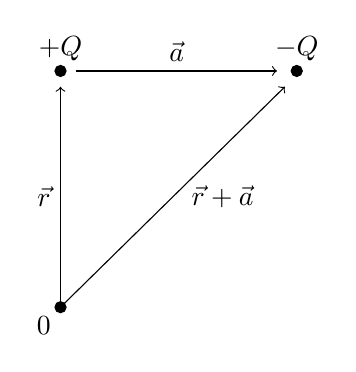
\begin{tikzpicture}
			
				 \draw[->](0,0)-- node[left]{$\vec{r}$} (0,2.8) ;
				 \draw[->](0,0)--node[right]{$\ \vec{r}+\vec{a}$}(2.85,2.8);
				 \draw[->](0.2,3)-- node[above]{$\vec{a}$}(2.75,3);
				 \filldraw[black] (0,0) circle (2pt) node[below left]{$0$};
				 \filldraw[black] (0,3) circle (2pt) node[above]{$+Q$};
				 \filldraw[black] (3,3) circle (2pt) node[above]{$-Q$};
			
			
			\end{tikzpicture}
		}
	}
	\caption{elektrischer Dipol}
\end{wrapfigure}
Ein Dipol besteht aus zwei gleich großen, entgegengesetzt geladenen Ladungen $\pm Q $, welche  einen festen Abstand $\vec{a}$ voneinander entfernt sind. Daher ergibt es Sinn, als charakteristische Eigenschaft des Dipols das \textbf{Dipolmoment} $\vec{p}$ wie folgt zu definieren:

\begin{equation*}
\vec{p} := Q \cdot \vec{a}
\end{equation*}

\begin{equation*}
\text{Dipollimit: } \quad |\vec{a}| \ \rightarrow \ 0, \ Q \ \rightarrow \ \infty 
\end{equation*}

\begin{equation*}
\Rightarrow \ |\vec{p}| = \ \text{const.}
\end{equation*}

Für das Potentialfeld eines solchen Dipols gilt offensichtlich:

\begin{equation*}
\varphi(\vec{r}) = \frac{Q}{4\pi\epsilon_0}\cdot\left(\frac{1}{|\vec{r}|} - \frac{1}{|\vec{r}+\vec{a}|}\right)
\end{equation*}

Für große Abstände von diesem Dipol, d.h. $\vec{r}\gg\vec{a}$ wollen wir das Potentialfeld \textsc{Taylor}-entwickeln, um besser mit ihm arbeiten zu können.\
Dazu betrachten wir den Term $\frac{1}{|\vec{r}+\vec{a}|}$ ein wenig genauer:\\

\begin{equation*}
\frac{1}{|\vec{r}+\vec{a}|} \cong \frac{1}{|\vec{r}|} + \left(\vec{a}\cdot\pdiff{}{\vec{r}}\right) \ \frac{1}{|\vec{r}|} = \frac{1}{|\vec{r}|}-\vec{a}\cdot\frac{\vec{r}}{|\vec{r}|^3}
\end{equation*}
\ \\
Damit gilt für das Potential:

\begin{equation*}
\varphi(\vec{r})=\frac{Q}{4\pi\epsilon_0}\left(\frac{1}{r}-\frac{1}{r}-\left(\vec{a}\cdot\pdiff{}{\vec{r}}\right)\frac{1}{r}\right) = \frac{\vec{p}\cdot\vec{r}}{4\pi\epsilon_o\cdot r^3}
\end{equation*}

und das $\vec{E}$-Feld:

\begin{align*}
\vec{E}(\vec{r}) &= - \nabla \varphi = \frac{1}{4\pi\epsilon_0}\ \nabla \left(\vec{p}\cdot\nabla\right)\ \frac{1}{r} = \frac{\vec{p}}{4\pi\epsilon_0}\ \underbrace{\left(\nabla \circ \nabla\right)\ \frac{1}{r}}_{(*)}\\
&= \frac{1}{4\pi\epsilon_0}\ \frac{3(\vec{p}\cdot\vec{r})\vec{r} - \vec{p}r^2}{r^5}\\
\ \\
\text{mit}\quad (*) &= \left(\pdiff{}{\vec{r}} \circ \pdiff{}{\vec{r}}\right)\frac{1}{|\vec{r}|} = - \pdiff{}{\vec{r}}\circ\frac{\vec{r}}{|\vec{r}|^3} = \frac{3\vec{r}\circ\vec{r}-\mathbbm{1}\cdot\vec{r}^2}{|\vec{r}|^5}
\end{align*}